\documentclass[border=2mm,
               tikz,
               preview]{standalone}
\usetikzlibrary{positioning,chains}

\begin{document}

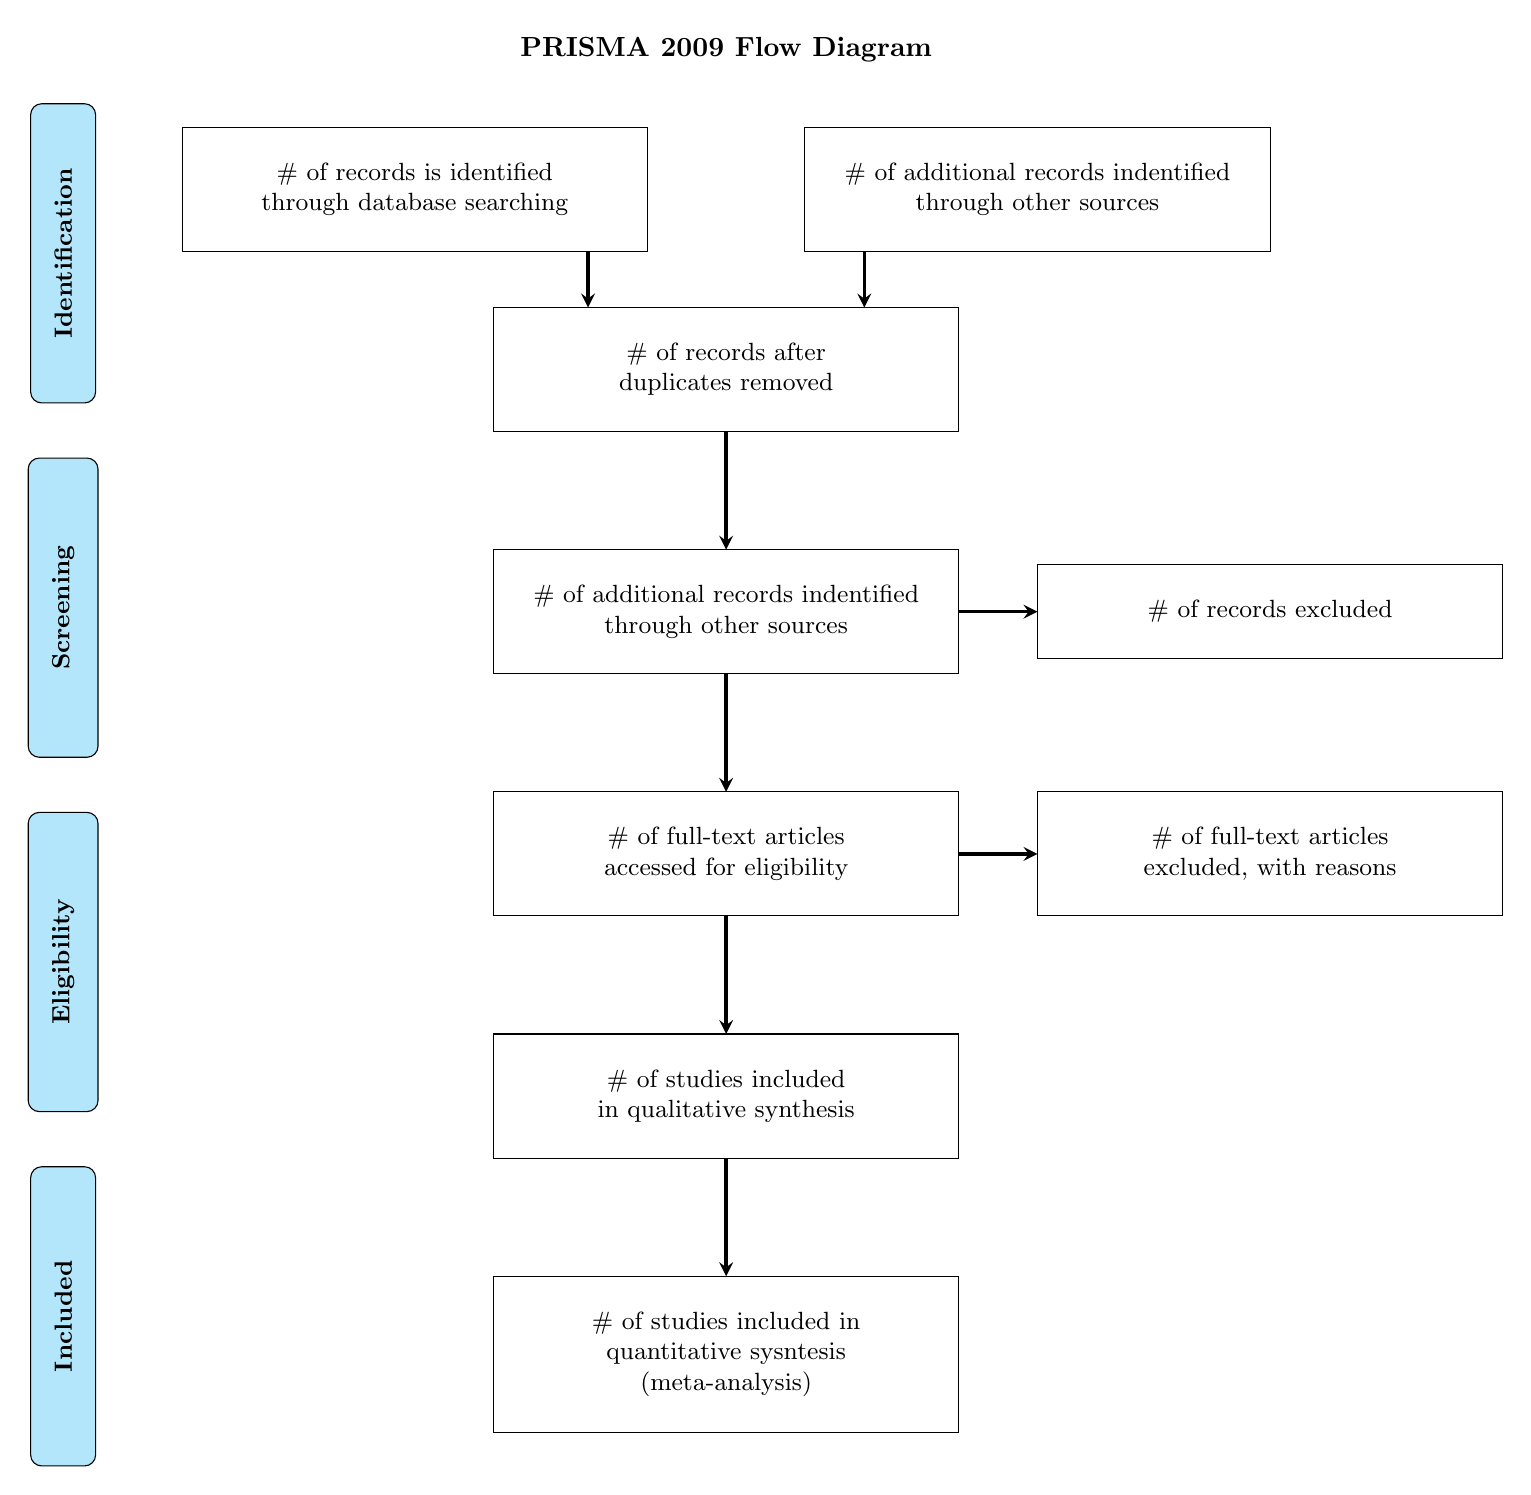
\begin{tikzpicture}[
    node distance=15mm and 10mm,
    start chain=going below,
 mynode/.style = {
        draw, rectangle, align=center, text width=5cm,
        font=\small, inner sep=3ex, outer sep=0pt,
        on chain},
mylabel/.style = {
        draw, rectangle, align=center, rounded corners, 
        font=\small\bfseries, inner sep=2ex, outer sep=0pt,
        fill=cyan!30, minimum height=38mm,
        on chain},
every join/.style = arrow,
     arrow/.style = {very thick,-stealth}
                    ] 
\coordinate (tc);
% the title
\node[above=of tc,font=\bfseries] {PRISMA 2009 Flow Diagram};
% the nodes at the top
\node (n1a) [mynode, left=of tc]    {\# of records is identified 
                                        through database searching};
\node (n1b) [mynode,right=of tc]    {\# of additional records indentified\\
                                        through other sources};
    % the chain in the center
\node (n2)  [mynode, below=of tc]   {\# of records after duplicates removed};
\node (n3)  [mynode,join]   {\# of additional records indentified\\
                                        through other sources};
\node (n4)  [mynode,join]   {\# of full-text articles accessed 
                                            for eligibility};
\node (n5)  [mynode,join]   {\# of studies included in qualitative synthesis};
\node (n6)  [mynode,join]   {\# of studies included in quantitative sysntesis\\
                                (meta-analysis)};
% the branches to the right
\node (n3r) [mynode,right=of n3]    {\# of records excluded};
\node (n4r) [mynode,right=of n4]    {\# of full-text articles excluded,
                                        with reasons};
% lines not included in join                                        
\draw[arrow] ([xshift=+22mm] n1a.south) coordinate (a)
                                       -- (a |- n2.north);
\draw[arrow] ([xshift=-22mm] n1b.south) coordinate (b)
                                       -- (b |- n2.north);
\draw[arrow] (n3) -- (n3r);
\draw[arrow] (n4) -- (n4r);
% the labels on the left
    \begin{scope}[node distance=7mm]
\node[mylabel,below left=-3mm and 11mm of n1a.north west]
                {\rotatebox{90}{Identification}};
\node[mylabel]  {\rotatebox{90}{Screening}};
\node[mylabel]  {\rotatebox{90}{Eligibility}};
\node[mylabel]  {\rotatebox{90}{Included}};
    \end{scope}
\end{tikzpicture}
\end{document}